% !TeX program = xelatex
\documentclass[a4paper,10pt]{article}

% ============================================================================
% កញ្ចប់បណ្ណាល័យ (Packages) – តាមលំនាំ NGS Preah Krasang Scenario
% ============================================================================
\usepackage[a4paper, left=0.95cm, right=0.95cm, top=0.80cm, bottom=0.90cm, footskip=0.45cm]{geometry}
\usepackage{amsmath}
\usepackage{unicode-math}
\usepackage{fontspec}
\usepackage{array, longtable, multirow, colortbl}
\usepackage[table]{xcolor}
\usepackage{enumitem}
\usepackage{pifont}
\usepackage{fancyhdr}
\usepackage{tikz}
\usetikzlibrary{calc, arrows.meta, decorations.markings, patterns, babel}

% LaTeX 2025 + longtable v4.24 compatibility guard
\makeatletter
\let\@expl@@@mark@update@singlecol@structures@@\relax
\makeatother

% ============================================================================
% ការកំណត់ពុម្ពអក្សរ (Fonts Configuration - Cross-Platform Windows + Cloud fonts/)
% ============================================================================
\providecommand{\NGSFindFonts}{%
  \IfFileExists{C:/Windows/Fonts/cambria.ttc}{%
    \def\NGSSysPath{C:/Windows/Fonts/}%
    \def\NGSUserPath{C:/Users/KIT/AppData/Local/Microsoft/Windows/Fonts/}%
  }{%
    \IfFileExists{./fonts/KhmerOSsiemreap.ttf}{\def\NGSSysPath{./fonts/}\def\NGSUserPath{./fonts/}}{%
    \IfFileExists{../fonts/KhmerOSsiemreap.ttf}{\def\NGSSysPath{../fonts/}\def\NGSUserPath{../fonts/}}{%
    \IfFileExists{../../fonts/KhmerOSsiemreap.ttf}{\def\NGSSysPath{../../fonts/}\def\NGSUserPath{../../fonts/}}{%
    \IfFileExists{../../../fonts/KhmerOSsiemreap.ttf}{\def\NGSSysPath{../../../fonts/}\def\NGSUserPath{../../../fonts/}}{%
    \IfFileExists{../../../../fonts/KhmerOSsiemreap.ttf}{\def\NGSSysPath{../../../../fonts/}\def\NGSUserPath{../../../../fonts/}}{%
    \IfFileExists{../../../../../fonts/KhmerOSsiemreap.ttf}{\def\NGSSysPath{../../../../../fonts/}\def\NGSUserPath{../../../../../fonts/}}{%
    \IfFileExists{../../../../../../fonts/KhmerOSsiemreap.ttf}{\def\NGSSysPath{../../../../../../fonts/}\def\NGSUserPath{../../../../../../fonts/}}{%
      \def\NGSSysPath{../../../../../../../fonts/}\def\NGSUserPath{../../../../../../../fonts/}%
    }}}}}}}%
  }%
}
\NGSFindFonts

\setmathfont[
  Path={\NGSSysPath},
  FontIndex=1,
  Scale=1.02
]{cambria.ttc}

\defaultfontfeatures{Ligatures=TeX}

\setmainfont[
  Path={\NGSUserPath},
  Extension=.ttf,
  Script=Khmer,
  BoldFont={KhmerOSsiemreap},
  BoldFeatures={FakeBold=1.8},
  ItalicFont={KhmerOSsiemreap},
  ItalicFeatures={FakeSlant=0.25},
  BoldItalicFont={KhmerOSsiemreap},
  BoldItalicFeatures={FakeBold=1.8, FakeSlant=0.25}
]{KhmerOSsiemreap}

\newfontfamily\muol[
  Path={\NGSUserPath},
  Extension=.ttf,
  Script=Khmer
]{KhmerOSmuollight}

\newfontfamily\TimesEn[
  Path={\NGSSysPath},
  Extension=.ttf,
  Scale=1.00,
  BoldFont={timesbd},
  ItalicFont={timesi},
  BoldItalicFont={timesbi}
]{times}

\newfontfamily\NagaBold[
  Path={\NGSUserPath},
  Extension=.ttf
]{AKbalthom Naga Bold}

\newfontfamily\CalibriFont[
  Path={\NGSSysPath},
  Extension=.ttf
]{calibri}

\newfontfamily\CourierBullet[
  Path={\NGSSysPath},
  Extension=.ttf
]{cour}
\newcommand{\wcirc}{{\CourierBullet\fontsize{9.5pt}{11pt}\selectfont o}}

\XeTeXlinebreaklocale "km"
\XeTeXlinebreakskip = 0pt plus 1pt minus 0.1pt

% ============================================================================
% ការកំណត់ពណ៌ និងទម្រង់ទំព័រ (Colors & Page Style)
% ============================================================================
\definecolor{stepgray}{HTML}{D9D9D9}
\definecolor{headgray}{HTML}{F2F2F2}
\definecolor{boxgray}{HTML}{D9D9D9}
\definecolor{darkred}{HTML}{C00000}
\definecolor{red5e}{HTML}{FF0000}

\pagestyle{fancy}
\fancyhf{}
\renewcommand{\headrulewidth}{0pt}
\fancyfoot[R]{\CalibriFont\fontsize{10.5pt}{12pt}\selectfont\thepage}

\setlength{\parindent}{0pt}
\setlength{\parskip}{0pt}
\setlength{\tabcolsep}{3.5pt}
\renewcommand{\arraystretch}{1.14}

\newcolumntype{L}[1]{>{\raggedright\arraybackslash}p{#1}}

% ============================================================================
% ម៉ាក្រូជំនួយ (Helper Macros)
% ============================================================================
\newcommand{\en}[1]{{\TimesEn #1}}
\newcommand{\enbf}[1]{{\TimesEn\textbf{#1}}}
\newcommand{\unit}[1]{\,\text{\en{#1}}}
\newcommand{\fiveE}[1]{{\NagaBold\fontsize{9.5pt}{13pt}\selectfont\textcolor{red5e}{#1}}}
\newcommand{\timenote}[1]{\textcolor{darkred}{\textit{#1}}}
\newcommand{\cnum}[1]{{\fontsize{10pt}{11.5pt}\selectfont\ding{\numexpr181+#1\relax}}}
\newcommand{\ditem}{\tikz[baseline=-0.5ex]\fill (0,0.38ex) -- (0.38ex,0) -- (0,-0.38ex) -- (-0.38ex,0) -- cycle;\hspace{0.25em}}

% រូបផ្ទៀងផ្ទាត់រហ័ស B&W (ដាក់ទន្ទឹមគ្នា ២ ផ្ទាំង ពេញទទឹង 18.8cm ស្អាតលើទំព័រទី ២)
\newcommand{\figScenarioRefPOWQ}{%
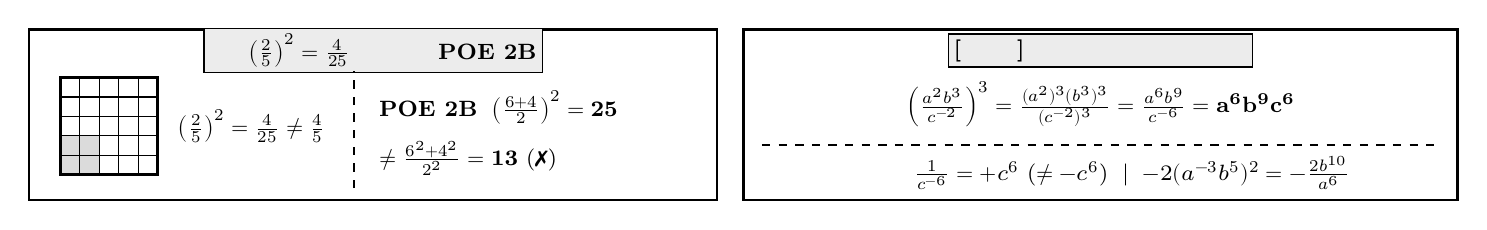
\begin{tikzpicture}[scale=0.95, every node/.style={font=\footnotesize, text=black}]
  % ផ្នែកឆ្វេង៖ ក្រឡា (2/5)^2 = 4/25 និង POE 2B អន្ទាក់ផលបូក
  \begin{scope}[shift={(0,0)}]
    \draw[black, line width=0.9pt] (0,0) rectangle (9.20,2.28);
    \node[fill=gray!15, draw=black, line width=0.5pt, inner sep=2pt] at (4.60,2.00) {\textbf{ក្រឡា} $\left(\frac{2}{5}\right)^2 = \frac{4}{25}$ \textbf{និង អន្ទាក់ \en{POE 2B}}};
    \begin{scope}[shift={(0.42,0.34)}]
      \fill[gray!28] (0,0) rectangle (0.52,0.52);
      \draw[black, line width=0.45pt] (0,0) grid[step=0.26] (1.30,1.30);
      \draw[black, line width=0.9pt] (0,0) rectangle (1.30,1.30);
      \node[anchor=west] at (1.44,0.65) {$\left(\frac{2}{5}\right)^2 = \frac{4}{25} \neq \frac{4}{5}$};
    \end{scope}
    \draw[black, line width=0.7pt, dashed] (4.35,0.16) -- (4.35,1.72);
    \node[anchor=west] at (4.55,1.24) {\textbf{\en{POE 2B}៖} $\left(\frac{6+4}{2}\right)^2 = \mathbf{25}$};
    \node[anchor=west] at (4.55,0.56) {$\neq \frac{6^2+4^2}{2^2} = \mathbf{13}$ (\ding{55})};
  \end{scope}

  % ផ្នែកស្ដាំ៖ [ចង្អុលអូស] និងប្រយ័ត្ន 1/c^{-6} = +c^6
  \begin{scope}[shift={(9.55,0)}]
    \draw[black, line width=0.9pt] (0,0) rectangle (9.55,2.28);
    \node[fill=gray!15, draw=black, line width=0.5pt, inner sep=2pt] at (4.775,2.00) {\textbf{[ចង្អុលអូស] ពីក្រៅចូលក្នុង និងច្រាសនិទស្សន្តដក}};
    \node at (4.775,1.28) {$\left(\frac{a^2 b^3}{c^{-2}}\right)^3 = \frac{(a^2)^3 (b^3)^3}{(c^{-2})^3} = \frac{a^6 b^9}{c^{-6}} = \mathbf{a^6 b^9 c^6}$};
    \draw[black, line width=0.7pt, dashed] (0.25,0.74) -- (9.30,0.74);
    \node at (4.775,0.36) {\textbf{ប្រយ័ត្ន៖} $\frac{1}{c^{-6}} = +c^6$ ($\neq -c^6$) \;\textbar{}\; $-2(a^{-3}b^5)^2 = -\frac{2b^{10}}{a^6}$};
  \end{scope}
\end{tikzpicture}}

\begin{document}
\fontsize{9.8pt}{14.6pt}\selectfont

% ============================================================================
% ក្បាលទំព័រ (Header & Metadata)
% ============================================================================
\begin{center}
{\muol\fontsize{10.4pt}{14pt}\selectfont សេណារីយ៉ូនៃការបង្រៀន \enbf{(}២\enbf{.}៤\enbf{.}៣ ស្វ័យគុណនៃផលចែក និងពង្រឹងលក្ខណៈទាំង ៣\enbf{)}}
\end{center}
\vspace{2pt}

\noindent{\setlength{\tabcolsep}{4pt}%
\begin{tabular}{|L{1.75cm}|L{6.65cm}|L{1.85cm}|L{7.55cm}|}
\hline
\rowcolor{headgray}
\textbf{សាលារៀន៖} & អនុវិទ្យាល័យព្រះក្រសាំង (កំពង់ស្វាយ--កំពង់ធំ) & \textbf{មុខវិជ្ជា៖} & គណិតវិទ្យា ថ្នាក់ទី៨ (ពីជគណិត) \\
\hline
\textbf{មេរៀន៖} & \textbf{២.៤.៣. ស្វ័យគុណនៃផលចែក និងពង្រឹងលក្ខណៈទាំង ៣} & \textbf{រយៈពេល៖} & \textcolor{darkred}{\textbf{១ ម៉ោងសិក្សា (៥០ នាទី)}} \textbullet\ ទំ.១៧–១៨, ២៥–២៦ \\
\hline
\textbf{គ្រូបង្រៀន៖} & ហុក ប៊ុនថែន & \textbf{កាលបរិច្ឆេទ៖} & ថ្ងៃចន្ទ ទី១៦ ខែវិច្ឆិកា ឆ្នាំ២០២៦ (៧កើត ខែកត្តិក ព.ស. ២៥៧០) \\
\hline
\end{tabular}}

\vspace{3pt}
{\muol ផ្នែកទី ១៖ លំដាប់ឈុតឆាកបង្រៀន ៥០ នាទី \enbf{(}៨ ឈុតលម្អិត\enbf{)}}
\vspace{1pt}

% ============================================================================
% ផ្នែកទី ១៖ តារាងឈុតឆាក (8 Chronological Scenes = 50 min, Granular Sub-Rows)
% ============================================================================
\begin{longtable}{|c|L{2.75cm}|c|L{7.65cm}|L{4.45cm}|}
\hline
\rowcolor{stepgray}
\textbf{ម៉ោង} & \textbf{ឈុត / ជំហាន \enbf{5E}} & \textbf{នាទី} & \textbf{សកម្មភាពបង្រៀន និងសំណួរ--ចម្លើយគំរូ (គ្រូ--សិស្ស)} & \textbf{សម្ភារៈ និងកំណត់ចំណាំ / \enbf{Warrant}} \\
\hline
\endfirsthead
\hline
\rowcolor{stepgray}
\textbf{ម៉ោង} & \textbf{ឈុត / ជំហាន \enbf{5E}} & \textbf{នាទី} & \textbf{សកម្មភាពបង្រៀន និងសំណួរ--ចម្លើយគំរូ (គ្រូ--សិស្ស)} & \textbf{សម្ភារៈ និងកំណត់ចំណាំ / \enbf{Warrant}} \\
\hline
\endhead
\hline
\endfoot
\hline
\endlastfoot

00--02 &
\textbf{ឈុតទី ១}\par
ជំហានទី១៖ រដ្ឋបាលថ្នាក់ &
២ &
\ditem គ្រូពិនិត្យអវត្តមាន និងបែងចែកសិស្សជា \textbf{«ក្រុមអ្នកស៊ើបអង្កេតស្វ័យគុណ ៣ តួនាទី»} (៣ នាក់/ក្រុម) ។\par
\ditem \textbf{គ្រូ៖} «ដាក់កន្ត្រៃ និងបន្ទាត់រាបស្មើលើតុ ហើយផ្កាប់សន្លឹក ១:១ មុនពេលចាប់ផ្ដើម!» \par
\textbf{សិស្ស៖} អនុវត្តតាម។ &
\wcirc\ កំណត់វិន័យកន្ត្រៃ/បន្ទាត់។\par
\wcirc\ ចែកសន្លឹក \en{P1 1:1} ផ្កាប់មុខ។ \\
\hline

02--08 &
\textbf{ឈុតទី ២}\par
ជំហានទី២៖ កំណែ និងរំលឹកមេរៀនចាស់ &
៦ &
\ditem \textbf{ក. កំណែ ($\le 3\unit{min}$, ប្រតិបត្តិ ៤.២ ទំ.១៨)៖}\par
ក. $-2(a^{-3}\cdot b^5)^2 = -2a^{-6}b^{10} = -\frac{2b^{10}}{a^6}$ ($a\neq 0$);\par
\textbf{គ្រូ៖} «ហេតុអ្វី $-2$ មិនលើកជា $(-2)^2 = +4$?» \par
\textbf{សិស្ស៖} «ព្រោះ $-2$ ស្ថិតនៅ\textbf{ក្រៅ}វង់ក្រចក!» &
\wcirc\ រក្សាកំណែ $\le 3$ នាទី។\par
\wcirc\ ផ្ដោតសញ្ញាដកក្រៅវង់ក្រចក (\cnum{5})។ \\[3pt]

& & &
\ditem ខ. $a\cdot(a^4)^5\cdot a^{-6} = a^{15}$ ($a\neq 0$) — បញ្ជាក់កំណត់សម្គាល់ពុម្ពទំ.១៨ ដែលបាត់និទស្សន្ត $5$ ក្លាយជា $a\cdot(a^4)\cdot a^{-6} = a^{-1} = \frac{1}{a}$ ។ &
\wcirc\ ប្រៀបធៀបពុម្ពទំ.១៧ vs ទំ.១៨ កុំឱ្យសិស្សភាន់ច្រឡំ។ \\[3pt]

& & &
\ditem \textbf{ខ. រំលឹក (៣នាទី)៖} §3 $\frac{a^m}{a^n}=a^{m-n},\; a^0=1,\; a^{-n}=\frac{1}{a^n}$ ($a\neq 0$); §4.1 $(a^m)^n=a^{mn}$; §4.2 $(ab)^n=a^nb^n$ ។ &
\wcirc\ \en{Warrant} \cnum{2}--\cnum{4}៖ រំលឹកច្បាប់មុនភ្ជាប់ផលចែក។ \\
\hline

08--11 &
\textbf{ឈុតទី ៣}\par
\fiveE{E1 Engage}\par
បង្រួមធុងស្តុកទឹកគូប &
៣ &
\ditem \textbf{«បេសកកម្មកាត់បង្រួមធុងស្តុកទឹក និងផ្ទាំងសំណាញ់នៅព្រះក្រសាំង»៖} បង្រួមគែមធុងគូប $1\unit{m}$ ($V_0 = 1\unit{m}^3$) មកត្រឹម $\frac{2}{5}\unit{m}$ ។\par
\ditem \textbf{គ្រូ (អន្ទាក់)៖} «សិស្សម្នាក់គណនា $\frac{2^3}{5} = \frac{8}{5} = 1.6\unit{m}^3$! តើធុងតូចជាងដើម អាចផ្ទុកទឹកច្រើនជាង $1\unit{m}^3$ បានទេ?» &
\wcirc\ បរិបទជាក់ស្ដែងព្រះក្រសាំង; សួរទស្សន៍ទាយមុន មិនទាន់លាតចម្លើយ។ \\[3pt]

& & &
\textbf{សិស្ស៖} ឆ្លើយជំទាស់ភ្លាមថា «មិនអាចធុងតូចផ្ទុកច្រើនជាងធុងដើមទេ!» តែនៅឆ្ងល់ចម្លើយពិត ។ គ្រូកត់ទុកលើក្ដារខៀនផ្ទៀងនៅ \fiveE{E5} ។ &
\wcirc\ កត់ត្រាការទស្សន៍ទាយទុកបិទបេសកកម្មនៅ \fiveE{E5} ។ \\
\hline

11--22 &
\textbf{ឈុតទី ៤}\par
\fiveE{E2 Explore}\par
ក្រឡា ១:១ និង \en{Dual POE} (\en{5m + 6m}) &
១១ &
\ditem \textbf{សកម្មភាព ១ (៥នាទី, \en{P1 1:1})៖} ផ្ទៀងក្រិត $5.00\unit{cm}$ (\en{Actual Size 100\%}), កាត់បន្ទះ $2.00\times 2.00\unit{cm}$ ដាក់លើក្រឡា $5.00\times 5.00\unit{cm}$ ($25$ ការ៉េ) ឃើញ $\left(\frac{2}{5}\right)^2 = \frac{4}{25} \neq \frac{4}{5}$ ។\par
\ditem \textbf{ផ្គុំកត្តា (ទំ.១៨)៖} ក. $\frac{2^3}{5^3}=\left(\frac{2}{5}\right)^3$; ខ. $\frac{a^n}{b^n}=\left(\frac{a}{b}\right)^n$ ។ &
\wcirc\ សន្លឹក \en{P1 1:1} ($5\times 5\unit{cm}$ + បន្ទះកាត់ $2\times 2\unit{cm}$)។\par
\wcirc\ រាប់ផ្ទាល់ $4$ ក្នុង $25$ ការ៉េ។ \\[3pt]

& & &
\ditem \textbf{សកម្មភាព ២ \en{Dual POE} — \en{POE 2A} (៣នាទី)៖} ក្រឡា $4.00\times 4.00\unit{cm}$ ($16$ ការ៉េ) ឈូស $3.00\times 3.00\unit{cm}$ $\implies$ ទស្សន៍ទាយមុនផ្ទៀង $\left(\frac{3}{4}\right)^2 = \frac{9}{16} \neq \frac{9}{4}$ ។ &
\wcirc\ ប្រៀបធៀបការទាយ $9/4 > 1$ vs ការ៉េឈូស $9$ ក្នុង $16$ ។ \\[3pt]

& & &
\ditem \textbf{\en{POE 2B} (៣នាទី — អន្ទាក់ផលបូក)៖} $\left(\frac{6+4}{2}\right)^2 = 5^2 = 25$ ធៀប $\frac{6^2+4^2}{2^2} = \frac{52}{4} = 13$ $\implies$ ស្វ័យគុណ\textbf{មិនចែកចាយ}លើ $+$ ឬ $-$ ឡើយ! &
\wcirc\ បង្កើតជម្លោះយល់ដឹង៖ ផ្គូផ្គងច្បាប់ផលចែកត្រូវទន្ទឹមអន្ទាក់ផលបូក។ \\
\hline

22--28 &
\textbf{ឈុតទី ៥}\par
\fiveE{E3 Explain}\par
ទ្រឹស្ដី ៤.៣ និង \en{Hub-and-Spoke} &
៦ &
\ditem សិស្សបង្គុំប្រអប់ \textbf{«ជាទូទៅ ៤.៣» (ទំ.១៨)}៖ $\left(\frac{a}{b}\right)^n = \frac{a^n}{b^n}$ ($a,b\neq 0, n\neq 0$) ព្រមទាំងទម្រង់\textbf{ពីរទិស} និងច្បាប់ច្រាស $\left(\frac{a}{b}\right)^{-n} = \left(\frac{b}{a}\right)^n$ ។ &
\wcirc\ \cnum{1} ពីរទិស និង $(a/b)^{-n}$ ។ \\[3pt]

& & &
\ditem បង្គុំដ្យាក្រាម \textbf{\en{Hub-and-Spoke}} ជុំវិញ $x^n$ តភ្ជាប់ §4.1, §4.2, §4.3 និងសង្ខេបតារាងសម្មតិកម្ម--សន្និដ្ឋាន--វិបាក ។ &
\wcirc\ ផ្ទាំង \textbf{\en{P4}}៖ \en{Hub-and-Spoke} + សំណួរ ៣ ជំហាន។ \\[3pt]

& & &
\ditem បិទផ្ទាំង \textbf{ធនាគារហេតុផល \cnum{1}--\cnum{5}}៖ \cnum{1} $\left(\frac{a}{b}\right)^n=\frac{a^n}{b^n}$, \cnum{2} $(ab)^n=a^nb^n$, \cnum{3} $(a^m)^n=a^{mn}$, \cnum{4} $a^m a^n, \frac{a^m}{a^n}, a^0, \frac{1}{c^{-n}}=c^n$, \cnum{5} $(-x)^{\text{គូ/សេស}}$ និង $(a\pm b)^n\neq a^n\pm b^n$ ។ &
\wcirc\ \cnum{4} $\frac{1}{c^{-n}}=+c^n$; \cnum{5} គូ/សេស និងហាម $+,-$ ។ \\
\hline

28--38 &
\textbf{ឈុតទី ៦}\par
\fiveE{E4 Elaborate}\par
កាត \textbf{[ចង្អុលអូស]} និង \en{EIA} &
១០ &
\ditem ចែកកាត \textbf{\en{P2 (2-up)}} អនុវត្ត ៣ ជំហាន (\textbf{[ចង្អុលអូស]} $\to$ \cnum{1}--\cnum{5} $\to$ គណនា)៖\par
• \textbf{គំរូ ១ ក (ទំ.១៨)៖} $\left(\frac{3}{4}\right)^3 = \frac{3^3}{4^3} = \frac{27}{64}$ (\cnum{1})\par
• \textbf{គំរូ ១ ខ (ទំ.១៨)៖} $\left(\frac{a^2b^3}{c^{-2}}\right)^3 = \frac{(a^2)^3(b^3)^3}{(c^{-2})^3} = \frac{a^6b^9}{c^{-6}} = a^6b^9c^6$ (\cnum{1}--\cnum{4}; $c\neq 0$) &
\wcirc\ \en{P2} បង្ហាញព្រួញ \textbf{[ចង្អុលអូស]} ពី $3$ ទៅលើ $a^2, b^3$ និង $c^{-2}$ ។ \\[3pt]

& & &
\ditem \textbf{\en{Reverse Consolidation} គ.៖} $\frac{6^4}{3^4}\cdot(2^{-1})^2 = \left(\frac{6}{3}\right)^4\cdot 2^{-2} = 2^4\cdot 2^{-2} = 2^2 = 4$ (\cnum{1}, \cnum{3}, \cnum{4}) ។\par
\ditem \textbf{\en{EIA Looking-Back} (30s)៖} ១) ហេតុអ្វី $\frac{1}{c^{-6}} = +c^6$ មិនមែន $-c^6$? ២) ហេតុអ្វី $\frac{6^4}{3^4} = 2^4$ មិនមែន $2^0$? &
\wcirc\ ផ្ទៀង \en{Warrant} \cnum{1} (ទិសបញ្ច្រាស), \cnum{3}, \cnum{4} (ត្រឡប់ $c^{-6}$ ជា $+c^6$)។ \\
\hline

38--48 &
\textbf{ឈុតទី ៧}\par
\fiveE{E5 Evaluate}\par
\en{Relay}, បិទ \en{E1}, កាត \en{A--D} &
១០ &
\ditem \textbf{\en{Relay} ៣ តួនាទី (៦នាទី, \en{P3 2-up})៖}\par
• \textbf{Task 1 (ប្រតិបត្តិ ក ទំ.១៨)៖} $\left(\frac{-2}{3}\right)^4 = \frac{(-2)^4}{3^4} = \frac{16}{81}$ (\cnum{1}, \cnum{5})\par
• \textbf{Task 2 (ប្រតិបត្តិ ខ ទំ.១៨)៖} $\left(\frac{a^4\cdot b^{-2}}{c^3}\right)^2 = \frac{a^8 b^{-4}}{c^6} = \frac{a^8}{b^4 c^6}$ (\cnum{1}--\cnum{4}; $b,c\neq 0$) &
\wcirc\ តួនាទី ១៖ \textbf{[ចង្អុលអូស]} + \en{Pause-Ask!}\par
\wcirc\ តួនាទី ២៖ \cnum{1}--\cnum{4} និងគណនា \\[3pt]

& & &
\ditem \textbf{Task 3 (សំយោគលក្ខណៈទាំង ៣)៖} $\left(\frac{-2x^3}{y^2}\right)^3\cdot\frac{y^7}{x^5} = \frac{-8x^9}{y^6}\cdot\frac{y^7}{x^5} = -8x^4 y$ (\cnum{1}--\cnum{5}) ។\par
\ditem \textbf{បិទបេសកកម្ម \en{E1}៖} $V = \left(\frac{2}{5}\right)^3 = \frac{8}{125}\unit{m}^3 = 0.064\unit{m}^3 < 1\unit{m}^3$ (សមហេតុផល!) &
\wcirc\ តួនាទី ៣៖ ផ្ទៀងសញ្ញា \cnum{5} និង លំដាប់ (\en{Pause-Review!})។ \\[3pt]

& & &
\ditem \textbf{កាត \en{A--D} \& \en{Exit Ticket} (៤នាទី, \en{P5})៖} លើ $\left(\frac{-3x^2}{y^{-4}}\right)^2$៖ \en{A:} $\frac{9x^4}{y^{-4}}$ (\ding{55} \cnum{1}), \en{B:} $9x^4y^2$ (\ding{55} \cnum{3}), \en{C:} $9x^4y^8$ (\ding{51}), \en{D:} $-9x^4y^8$ (\ding{55} \cnum{5}) + សំបុត្រចេញ ៣ សំណួរ (៦០–៩០s) ។ &
\wcirc\ ត្រួតពិនិត្យកាត \en{A--D} ភ្លាម និងប្រមូលសំបុត្រចេញ។ \\
\hline

48--50 &
\textbf{ឈុតទី ៨}\par
ជំហានទី៥៖ កិច្ចការផ្ទះ &
២ &
\ditem ប្រគល់ប័ណ្ណកិច្ចការផ្ទះ \textbf{\en{P6}}៖\par
• \textbf{ផ្នែក ក (ទំ.១៨ \& ២៥ \#6 គ)៖} (១) $\left(\frac{-3}{5}\right)^3 = -\frac{27}{125}$; (២) $\left(\frac{2x^3y^{-1}}{z^4}\right)^3 = \frac{8x^9}{y^3z^{12}}$; (៣) $\left(\frac{4}{3}\right)^4\left(\frac{4}{3}\right)^{-6}\left(\frac{4}{3}\right)^3 = \frac{4}{3}$ ។\par
• \textbf{ផ្នែក ខ (ទំ.២៥ \#7 ង \& ទំ.២៦ \#8 ក, គ)៖} (១) $\frac{(32a^2x^8)^3}{(5ax)(-2a^2x^2)^2(-4a^3x)^3} = -\frac{128x^{16}}{5a^8}$; (២) $x^{12}=(x^2)^6$, $2^{18}=8^6$, $(2^5)^6=8^{10}$ ។ &
\wcirc\ ផ្ទៀងលេខលំហាត់លើ \en{P6} (សម្គាល់ទំ.២៦ ខ្វះ «.» ក្រោយ «គ»)។\par
\wcirc\ អានមុន៖ \textbf{៤.៤. ស្វ័យគុណនៃ \en{10} (ទំ.១៩–២០)} ។ \\
\hline
\end{longtable}

\vspace{1pt}
% ============================================================================
% ផ្នែកទី ២៖ បញ្ជីសម្ភារៈ B&W និងរូបផ្ទៀងផ្ទាត់រហ័ស (ហូរចូលទំព័រទី ២ ពេញស្អាត)
% ============================================================================
{\muol ផ្នែកទី ២៖ បញ្ជីសម្ភារៈ \enbf{B\&W} និងរូបផ្ទៀងផ្ទាត់រហ័ស}\\[2pt]
{\fontsize{8.5pt}{11.8pt}\selectfont
\ditem \textbf{\en{P1} (\en{1:1})៖} ក្រិត $5.00\unit{cm}$ (\en{Actual Size 100\%}), ក្រឡា $5\times 5\unit{cm}$ + បន្ទះកាត់ $2\times 2\unit{cm}$, \en{POE 2A} ($4\times 4\unit{cm}$), ប្រអប់ \en{POE 2B} \textbar{} \textbf{ឧបករណ៍៖} កន្ត្រៃ បន្ទាត់ \en{1:1} ខ្មៅដៃ \textbf{[ចង្អុលអូស]} ។\par
\ditem \textbf{\en{P2--P6}៖} កាត \en{E4} (\en{P2}), \en{Relay E5} (\en{P3}), ផ្ទាំង \en{Hub-and-Spoke} \& \textbf{\en{Warrant Bank} \cnum{1}--\cnum{5}} (\en{P4}), កាត \en{A--D} + \en{Exit Ticket} (\en{P5}), ប័ណ្ណកិច្ចការផ្ទះ (\en{P6}) ។\par
\ditem \textbf{ចំណាំ \en{Warrant}៖} \cnum{1} $\left(\frac{a}{b}\right)^n=\frac{a^n}{b^n}$ \textbar{} \cnum{2} $(ab)^n=a^n b^n$ \textbar{} \cnum{3} $(a^m)^n=a^{mn}$ \textbar{} \cnum{4} $a^m a^n, a^0, \frac{1}{c^{-n}}=c^n$ \textbar{} \cnum{5} គូ/សេស, $(a\pm b)^n\neq a^n\pm b^n$ ។\par}
\vspace{2pt}
\noindent{\centering\figScenarioRefPOWQ\par}

\vspace{6pt}
% ============================================================================
% ផ្នែកទី ៣៖ ការភាន់ច្រឡំសិស្ស និងវិធានការដោះស្រាយ (Full-Width Clean Table)
% ============================================================================
{\muol ផ្នែកទី ៣៖ ការភាន់ច្រឡំសិស្ស និងវិធានការដោះស្រាយ}\\[4pt]
{\fontsize{9.2pt}{13.6pt}\selectfont\renewcommand{\arraystretch}{1.22}%
\begin{tabular}{|L{7.65cm}|L{10.90cm}|}
\hline
\rowcolor{stepgray}
\textbf{ការភាន់ច្រឡំសិស្ស (\en{Empirical})} & \textbf{វិធានការបង្ការ និងដោះស្រាយក្នុងថ្នាក់} \\
\hline
\textbf{១. ភ្លេចភាគបែង / ដកនិទស្សន្តផលចែក៖} សរសេរ $(2/5)^3 = 2^3/5$ ឬ $9^3/3^3 = 3^0$ (\en{Ulusoy, 2019}: មានតែ 37.6\% ត្រូវ \en{Q10}, 17.0\% \en{Q9}) ។ & ប្រើ \textbf{\en{E1}} ធុងទឹក $1.6>1\unit{m}^3$, ក្រឡា \textbf{\en{P1 1:1}} ($4/25$ និង $9/16$), ដ្យាក្រាម \textbf{[ចង្អុលអូស]} (\en{P2}), និងកាតអន្ទាក់ \textbf{\en{A}} (\en{P5}) ។ \\
\hline
\textbf{២. បំបែកស្វ័យគុណលើផលបូក៖} គិតថា $(a+b)^n = a^n+b^n$ (\en{Fitria et al., 2023}: 66.2\%; \en{Kshetree et al., 2021}; \en{Van Dooren et al., 2003}: 13\% $\to$ 36\%) ។ & ផ្គូផ្គង \textbf{\en{POE 2B}} ($\left(\frac{6+4}{2}\right)^2=25 \neq 13$) ទន្ទឹមនឹងច្បាប់ផលចែក \cnum{1} តាំងពីដំបូង និងសំណួរ \en{Exit Ticket \#3} ។ \\
\hline
\textbf{៣. សញ្ញាដកក្រៅវង់ក្រចក និង គូ/សេស៖} ច្រឡំ $-2(a^{-3}b^5)^2$ ឬ $(-3x^2/y^{-4})^2$ (\en{Olson et al., 2011}: 5/19 [26.3\%]; \en{Ulusoy, 2019}: 66.1\% \en{Q1}) ។ & ញែក $-2[a^{-3}b^5]^2$ នៅកំណែ \en{Step 2}, ប្រើ \cnum{5} លើ \en{Task 1 \& 3} (\en{P3}), \en{Pause-Review!}, និងកាត \textbf{\en{C vs D}} (\en{P5}) ។ \\
\hline
\textbf{៤. និទស្សន្តដកភាគបែង និង លាយរូបមន្ត៖} ច្រឡំ $1/c^{-6}=-c^6$ ឬបូកជំនួសគុណ (\en{Ulusoy, 2019}: 63.6\%; \en{Rohrer et al., 2020}: 60.7\% vs 37.6\%) ។ & គូស \textbf{[ចង្អុលអូស]} (\en{Yeo \& Tzeng, 2019}), \en{Warrant} \cnum{1}--\cnum{5} (\en{Vest et al., 2022}), \en{EIA 30s}, និងលំហាត់ចម្រុះ \en{P6} ។ \\
\hline
\end{tabular}}

\vspace{8pt}
% ============================================================================
% ផ្នែកទី ៤៖ ប្លង់គ្រប់គ្រងក្ដារខៀន ៣ ភាគ (Board Management Plan)
% ============================================================================
{\muol ផ្នែកទី ៤៖ ប្លង់គ្រប់គ្រងក្ដារខៀន ៣ ភាគ}\\[3pt]
{\fontsize{8.8pt}{12.8pt}\selectfont\renewcommand{\arraystretch}{1.16}%
\begin{tabular}{|L{6.00cm}|L{6.25cm}|L{6.00cm}|}
\hline
\rowcolor{stepgray}
\textbf{ក្ដារខៀនឆ្វេង៖ ទ្រឹស្ដី ៤.៣, \en{Hub-and-Spoke} \& \cnum{1}--\cnum{5}} &
\textbf{ក្ដារខៀនកណ្ដាល៖ ពិសោធន៍ \en{E2} និងគំរូ \en{E4}} &
\textbf{ក្ដារខៀនស្ដាំ៖ \en{E1, Relay E5} និងបិទមេរៀន} \\
\hline
\textbf{៤.៣ ស្វ័យគុណនៃផលចែក (ទំ.១៨)៖}\par
$\left(\dfrac{a}{b}\right)^n = \dfrac{a^n}{b^n} \iff \dfrac{a^n}{b^n} = \left(\dfrac{a}{b}\right)^n$ \quad (\cnum{1})\par
$\left(\dfrac{a}{b}\right)^{-n} = \left(\dfrac{b}{a}\right)^n$ \quad ($a,b\neq 0,\; n\neq 0$)\par
\textbf{ពង្រឹងលក្ខណៈទាំង ៣ (\en{Hub} $x^n$)៖}\par
\cnum{3} $(a^m)^n=a^{mn}$ \textbar{} \cnum{2} $(ab)^n=a^nb^n$ \textbar{} \cnum{1} $\left(\frac{a}{b}\right)^n=\frac{a^n}{b^n}$\par
\cnum{4} $a^m a^n=a^{m+n},\; \frac{a^m}{a^n}=a^{m-n},\; a^0=1,\; \frac{1}{c^{-n}}=c^n$\par
\cnum{5} $(-x)^{\text{គូ}}=+x^{\text{គូ}},\; (-x)^{\text{សេស}}=-x^{\text{សេស}},\; (a\pm b)^n\neq a^n\pm b^n$
&
\textbf{ពិសោធន៍ \en{1:1} និង \en{Dual POE} (\en{E2})៖}\par
• $\left(\frac{2}{5}\right)^2 = \frac{4}{25} \neq \frac{4}{5}$ \textbar{} $\frac{2^3}{5^3} = \left(\frac{2}{5}\right)^3$\par
• \en{2A:} $\left(\frac{3}{4}\right)^2 = \frac{9}{16} \neq \frac{9}{4}$ \textbar{} \en{2B:} $\left(\frac{6+4}{2}\right)^2=25 \neq 13$\par
\textbf{លំហាត់គំរូទី ១ (\en{E4} [ចង្អុលអូស])៖}\par
• ក. $\left(\frac{3}{4}\right)^3 = \frac{27}{64}$\par
• ខ. $\left(\frac{a^2b^3}{c^{-2}}\right)^3 = \frac{a^6b^9}{c^{-6}} = a^6b^9c^6$ ($c\neq 0$)\par
• គ. $\frac{6^4}{3^4}\cdot(2^{-1})^2 = 2^4\cdot 2^{-2} = 4$
&
\textbf{បេសកកម្ម \en{E1} (ធុងទឹកគូបព្រះក្រសាំង)៖}\par
• ទាយខុស $\frac{2^3}{5}=1.6>1\unit{m}^3$ $\to$ ពិត $\left(\frac{2}{5}\right)^3 = \frac{8}{125}\unit{m}^3$!\par
\textbf{លទ្ធផល \en{Relay E5} (ទំ.១៨)៖}\par
• \en{T1:} $\left(\frac{-2}{3}\right)^4=\frac{16}{81}$ \textbar{} \en{T2:} $\left(\frac{a^4b^{-2}}{c^3}\right)^2=\frac{a^8}{b^4c^6}$\par
• \en{T3:} $\left(\frac{-2x^3}{y^2}\right)^3\cdot\frac{y^7}{x^5} = -8x^4y$ ($x,y\neq 0$)\par
\textbf{ត្រួតពិនិត្យ \en{A--D} និង \en{P6}៖}\par
ចម្លើយត្រូវ \en{C} ($9x^4y^8$) \textbar{} កិច្ចការផ្ទះ៖ ទំ.១៨, ២៥–២៦ \\
\hline
\end{tabular}}

\end{document}
